% Seção 6: Medição da temperatura ambiente

\section{Medição da temperatura ambiente}

A temperatura ambiente é medida por um sensor DS18B20 em sonda de aço inoxidável à prova d'água, com cabo de 90\,cm. O DS18B20 é um sensor digital: o elemento sensor, o conversor A/D e a interface de comunicação estão integrados no próprio encapsulamento, e a leitura é transmitida ao Arduino pelo barramento 1-Wire. Por isso, o circuito externo se resume à alimentação, a um resistor de \textit{pull-up} e a um capacitor de desacoplamento (Figura~\ref{fig:esq_ds18b20}).

\begin{figure}[H]
  \centering
  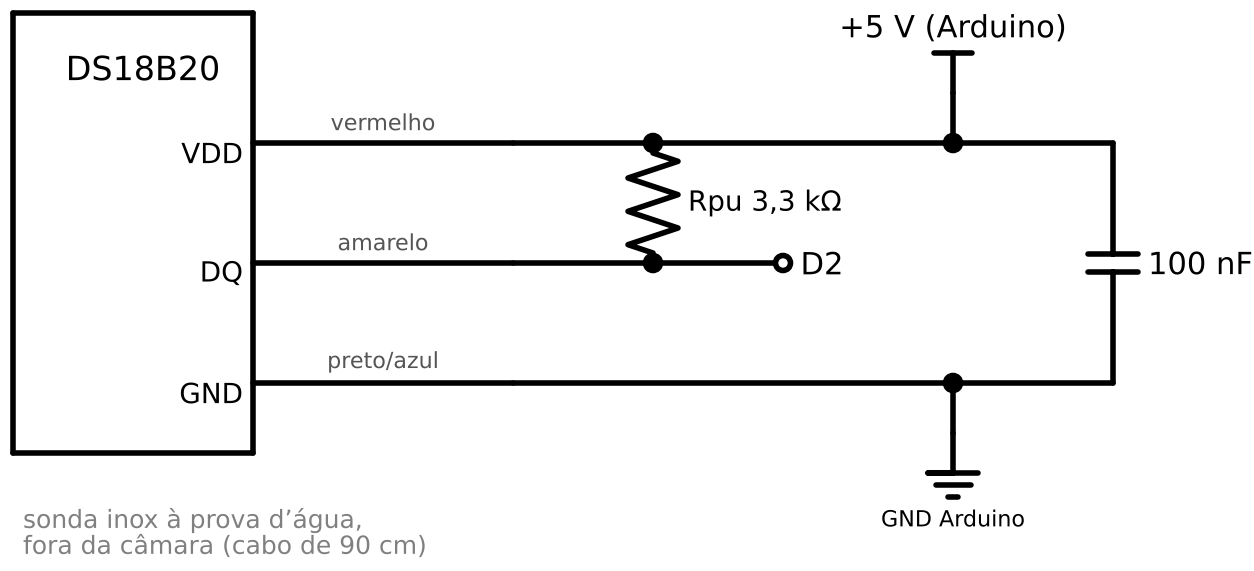
\includegraphics[width=0.75\textwidth]{esq_ds18b20.png}
  \caption{Ligação do sensor DS18B20 ao Arduino: alimentação em 5\,V, linha de dados (DQ) no pino digital D2 com resistor de \textit{pull-up} de 3,3\,k$\Omega$ e capacitor de desacoplamento de 100\,nF.}
  \label{fig:esq_ds18b20}
\end{figure}

\paragraph{Ligação.} O fio vermelho é ligado ao +5\,V, o fio de dados ao pino digital D2 e o fio de terra ao GND do Arduino. Como a sonda utilizada tem fios vermelho, azul e preto, o fio de terra é confirmado com o multímetro no modo diodo antes da primeira energização, já que a inversão entre alimentação e terra danifica o sensor. A linha de dados é de dreno aberto e precisa de um resistor de \textit{pull-up}; foi usado 3,3\,k$\Omega$, valor disponível no laboratório e adequado ao comprimento do cabo.

\paragraph{Características.} O sensor opera de $-$55 a 125\,\ensuremath{^\circ}C, com exatidão de $\pm$0,5\,\ensuremath{^\circ}C entre $-$10 e 85\,\ensuremath{^\circ}C. Com resolução de 12 bits, o passo de leitura é de 0,0625\,\ensuremath{^\circ}C e o tempo de conversão é de até 750\,ms. Como a temperatura ambiente varia em escala de minutos, uma leitura por segundo é suficiente para a compensação da perturbação. A conversão será disparada sem bloqueio (\textit{non-blocking}) pelas bibliotecas OneWire e DallasTemperature, de modo que a espera de 750\,ms não interrompa a malha de controle. Como a leitura é digital, ela não depende da referência do conversor A/D nem sofre interferência do PWM ao longo do cabo.

\paragraph{Posicionamento.} A sonda fica suspensa no ar a cerca de 20\,cm da câmara, longe da fonte e das passagens de cabos, para não medir o calor que escapa da câmara.
